\documentclass{standalone}
  \usepackage{tikz}
  \usetikzlibrary{arrows.meta, automata, bending, positioning, shapes.misc}
  \tikzstyle{automaton}=[shorten >=1pt, >={Stealth[bend,round]}, initial text=]
  \tikzstyle{accepting}=[accepting by arrow]

\begin{document}
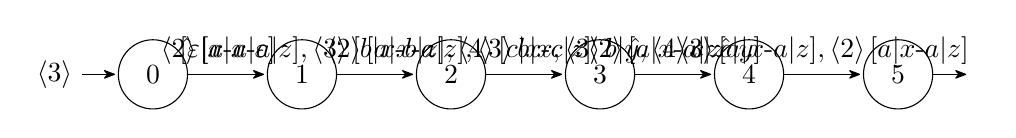
\begin{tikzpicture}[automaton, auto]
  \node[state,initial,initial text=$\left\langle 3\right\rangle$] (0) {$0$};
  \node[state] (1) [right=of 0] {$1$};
  \node[state] (2) [right=of 1] {$2$};
  \node[state] (3) [right=of 2] {$3$};
  \node[state] (4) [right=of 3] {$4$};
  \node[state,accepting] (5) [right=of 4] {$5$};
  \path[->] (0) edge node {$[\hat{}\varepsilon|x\textrm{-}a|\varepsilon]$} (1);
  \path[->] (1) edge node {$\left\langle 2\right\rangle [a|x\textrm{-}a|z], \left\langle 3\right\rangle [b|x\textrm{-}b|z], \left\langle 4\right\rangle [c|x\textrm{-}c|z]$} (2);
  \path[->] (2) edge node {$\left\langle 2\right\rangle [a|x\textrm{-}a|z], \left\langle 3\right\rangle b|x, \left\langle 3\right\rangle b|y, \left\langle 4\right\rangle c|z$} (3);
  \path[->] (3) edge node {$\left\langle 2\right\rangle [\hat{}a|x\textrm{-}a|zc|y]$} (4);
  \path[->] (4) edge node {$\left\langle 3\right\rangle [\hat{}a|x\textrm{-}a|z], \left\langle 2\right\rangle [a|x\textrm{-}a|z]$} (5);
\end{tikzpicture}
\end{document}
